%%%%%%%%%%%%%%%%%%%%%%%%%%%%%%%%%%%%%%%%%%%%%%%%%%%%%%%%%%%%%%%%%%%%%%%%%%%%%%%
%
% Filename: ira-analysis.tex
% Author:   David Oniani
% Modified: October 02, 2019
%  _         _____   __  __
% | |    __ |_   _|__\ \/ /
% | |   / _` || |/ _ \\  /
% | |__| (_| || |  __//  \
% |_____\__,_||_|\___/_/\_\
%
%%%%%%%%%%%%%%%%%%%%%%%%%%%%%%%%%%%%%%%%%%%%%%%%%%%%%%%%%%%%%%%%%%%%%%%%%%%%%%%

%%%%%%%%%%%%%%%%%%%%%%%%%%%%%%%%%%%%%%%%%%%%%%%%%%%%%%%%%%%%%%%%%%%%%%%%%%%%%%%
% Document definition
%%%%%%%%%%%%%%%%%%%%%%%%%%%%%%%%%%%%%%%%%%%%%%%%%%%%%%%%%%%%%%%%%%%%%%%%%%%%%%%

\documentclass[12pt]{article}

%%%%%%%%%%%%%%%%%%%%%%%%%%%%%%%%%%%%%%%%%%%%%%%%%%%%%%%%%%%%%%%%%%%%%%%%%%%%%%%
% Packages and related settings
%%%%%%%%%%%%%%%%%%%%%%%%%%%%%%%%%%%%%%%%%%%%%%%%%%%%%%%%%%%%%%%%%%%%%%%%%%%%%%%

% Global, document-wide settings
\usepackage[margin=1in]{geometry}
\usepackage[utf8]{inputenc}
\usepackage[english]{babel}

% Bibliography and references
\usepackage[backend=biber]{biblatex}
\addbibresource{$BIB}

% Math and alignment
\usepackage{multicol}
\usepackage{bookmark}
\usepackage{adjustbox}
\usepackage{braket}
\usepackage{mathtools}
\usepackage{amsmath}
\usepackage{amssymb}
\usepackage{amsthm}
\usepackage{amsfonts}
\usepackage{algorithmic}

% Graphics
\usepackage{pgfplots}
\pgfplotsset{compat=1.16}
\usepackage{tikz}
\usetikzlibrary{cd, arrows, decorations.markings}
\usepackage{graphicx}
\usepackage{rotating}
\usepackage{pst-solides3d}
\usepackage{xcolor}

% Fancy stuff
\usepackage{fancyhdr}
\usepackage{tocloft}
\usepackage{caption}
\usepackage{soul}
\usepackage{textcomp}
\usepackage{wasysym}
\usepackage[cache=false]{minted}
\usepackage{csquotes}
\usepackage{hyperref}

%%%%%%%%%%%%%%%%%%%%%%%%%%%%%%%%%%%%%%%%%%%%%%%%%%%%%%%%%%%%%%%%%%%%%%%%%%%%%%%
% Mathematican operations and operators
%%%%%%%%%%%%%%%%%%%%%%%%%%%%%%%%%%%%%%%%%%%%%%%%%%%%%%%%%%%%%%%%%%%%%%%%%%%%%%%

% Sets and related operators
\newcommand{\nats}{\mathbb{N}}                   % Natural numbers
\newcommand{\pnats}{\mathbb{N}^+}                % Positive natural numbers

\newcommand{\ints}{\mathbb{Z}}                   % Integers
\newcommand{\pints}{\mathbb{Z}^+}                % Positive integers
\newcommand{\nints}{\mathbb{Z}^-}                % Negative integers

\newcommand{\rats}{\mathbb{Q}}                   % Rational numbers
\newcommand{\prats}{\mathbb{Q}^+}                % Positive rational numbers
\newcommand{\nrats}{\mathbb{Q}^-}                % Negative rational numbers

\newcommand{\reals}{\mathbb{R}}                  % Real numbers
\newcommand{\preals}{\mathbb{R}^+}               % Positive real numbers
\newcommand{\nreals}{\mathbb{R}^-}               % Negative real numbers

\newcommand{\irrats}{\mathbb{I}}                 % Irrational numbers

\newcommand{\pset}{\mathcal{P}}                  % Powerset
\newcommand{\card}{\abs}                         % Cardinality
\newcommand{\topology}{\mathcal{T}}              % Topology
\newcommand{\basis}{\mathcal{B}}                 % Basis
\newcommand{\oldemptyset}{\emptyset}             % Old empty set
\renewcommand{\emptyset}{\varnothing}            % New and nice empty set

% Other operators
\DeclarePairedDelimiter\abs{\lvert}{\rvert}      % Absolute value
\DeclarePairedDelimiter\ceil{\lceil}{\rceil}     % Ceiling
\DeclarePairedDelimiter\floor{\lfloor}{\rfloor}  % Floor

%%%%%%%%%%%%%%%%%%%%%%%%%%%%%%%%%%%%%%%%%%%%%%%%%%%%%%%%%%%%%%%%%%%%%%%%%%%%%%%
% Command definitions and redefinitions
%%%%%%%%%%%%%%%%%%%%%%%%%%%%%%%%%%%%%%%%%%%%%%%%%%%%%%%%%%%%%%%%%%%%%%%%%%%%%%%

% New commands
\newcommand{\rarr}{\rightarrow}                        % Leftarrow
\newcommand{\larr}{\leftarrow}                         % Rightarrow
\newcommand\und[1]{\underline{\smash{#1}}}             % Nice-looking underline

% Renewed commands
\renewcommand{\headrulewidth}{0.5pt}                   % Header rule width
\renewcommand{\footrulewidth}{0pt}                     % Footer rule width
\renewcommand{\baselinestretch}{1.5}                   % Line spacing is 1.5
\renewcommand{\cftsecleader}{\cftdotfill{\cftdotsep}}  % Dots for ToC sections

% Rename "Contents" to "Table of Contents"
\addto\captionsenglish{% Replace "english" with the language used
  \renewcommand{\contentsname}%
    {\textbf{Table of Contents}}}%

% Filling the space for centering the title of the table of contents
\renewcommand{\cfttoctitlefont}{\hspace*{\fill}\Large}
\renewcommand{\cftaftertoctitle}{\hspace*{\fill}}

%%%%%%%%%%%%%%%%%%%%%%%%%%%%%%%%%%%%%%%%%%%%%%%%%%%%%%%%%%%%%%%%%%%%%%%%%%%%%%%
% Miscellaneous
%%%%%%%%%%%%%%%%%%%%%%%%%%%%%%%%%%%%%%%%%%%%%%%%%%%%%%%%%%%%%%%%%%%%%%%%%%%%%%%

% Setting stuff
\setlength{\parindent}{0pt}  % Remove indentations from paragraphs
\frenchspacing               % Get rid of large spaces after dots
\pagestyle{fancy}            % This allows to do fancy headers and footers
\fancyhf{}                   % No additional page numbering (or other stuff)
\cfoot{\thepage}             % Display page number at the bottom, in the center

% PDF information and nice-looking urls
\hypersetup{%
  pdfauthor  = {David Oniani},
  pdftitle   = {Textual and Statistical Analysis of Russian IRA Facebook Posts},
  pdfsubject = {Statistics, Authorship Attribution, Visual Persuasion},
  colorlinks = true,
  linkcolor  = {blue!50!black},
  citecolor  = {blue!50!black},
  urlcolor   = {blue!50!black}
}

% Put a centered header of a footnote size on the top of each page
\chead{\footnotesize{\MakeUppercase{Textual and Statistical Analysis of Russian IRA Facebook Posts}}}

% Definition environment
\theoremstyle{definition}
\newtheorem*{definition}{Definition}

%%%%%%%%%%%%%%%%%%%%%%%%%%%%%%%%%%%%%%%%%%%%%%%%%%%%%%%%%%%%%%%%%%%%%%%%%%%%%%%
% Author(s), title, and date
%%%%%%%%%%%%%%%%%%%%%%%%%%%%%%%%%%%%%%%%%%%%%%%%%%%%%%%%%%%%%%%%%%%%%%%%%%%%%%%

% Author(s)
\author{David Oniani\\
        Luther College\\
        \href{mailto:oniada01@luther.edu}{oniada01@luther.edu}}

% Title
\title{\textbf{Textual and Statistical Analysis of Russian IRA Facebook Posts}\\
      \small \textsuperscript{*}The paper is written in the scope of a student-faculty collaborative\\
                                summer research with professor Richard K. Merritt.}

% Date
\date{Month Day, Year}

%%%%%%%%%%%%%%%%%%%%%%%%%%%%%%%%%%%%%%%%%%%%%%%%%%%%%%%%%%%%%%%%%%%%%%%%%%%%%%%
% Beginning of the document
%%%%%%%%%%%%%%%%%%%%%%%%%%%%%%%%%%%%%%%%%%%%%%%%%%%%%%%%%%%%%%%%%%%%%%%%%%%%%%%

\begin{document}
\maketitle

%%%%%%%%%%%%%%%%%%%%%%%%%%%%%%%%%%%%%%%%%%%%%%%%%%%%%%%%%%%%%%%%%%%%%%%%%%%%%%%
% Abstract
%%%%%%%%%%%%%%%%%%%%%%%%%%%%%%%%%%%%%%%%%%%%%%%%%%%%%%%%%%%%%%%%%%%%%%%%%%%%%%%

\begin{abstract}
\addcontentsline{toc}{section}{Abstract}

\noindent The 2016 United States Presidential Election was targeted by an
unprecedented intelligence and influence campaign. Arising out of Russian
so-called Internet Research Agency (IRA), it sought to sow discord and attack
the fissures of the United States with the ultimate goal of swaying the
election results.~\cite{ira2016}~\cite{ira2016data} Recently, some of the
IRA-backed Facebook advertisements were released by The United States House
Permanent Select Committee on Intelligence. All of the advertisements are in
the PDF format. We have scraped the PDF files and present the results obtained
by textual and statistical analysis of the above-mentioned data. Authorship
attribution and sentiment analysis tests were also performed.~\footnote{Please
note that this paper does not discuss neither social, nor political implications
of these events, but attempts to explore the methods of persuasion that were
employed in this influence campaign.}~\cite{ira2016csvdata} We have also made
the data publicly available for other researchers and/or interested people in
a much nicer and easier-to-manipulate CSV format.
\end{abstract}

%%%%%%%%%%%%%%%%%%%%%%%%%%%%%%%%%%%%%%%%%%%%%%%%%%%%%%%%%%%%%%%%%%%%%%%%%%%%%%%
% Table of Contents
%%%%%%%%%%%%%%%%%%%%%%%%%%%%%%%%%%%%%%%%%%%%%%%%%%%%%%%%%%%%%%%%%%%%%%%%%%%%%%%

\newpage
\tableofcontents
\newpage

%%%%%%%%%%%%%%%%%%%%%%%%%%%%%%%%%%%%%%%%%%%%%%%%%%%%%%%%%%%%%%%%%%%%%%%%%%%%%%%
% Data and Preparation
%%%%%%%%%%%%%%%%%%%%%%%%%%%%%%%%%%%%%%%%%%%%%%%%%%%%%%%%%%%%%%%%%%%%%%%%%%%%%%%

\section*{\centering Data and Preparation}
\addcontentsline{toc}{section}{Data and Preparation}

The dataset was scraped from~\cite{ira2016data} more than 3500 Russian IRA
Facebook posts made publicly available in the PDF format by the House
Intelligence Committee. We used the free and open-source Python library
~\cite{pdftotext} \texttt{pdftotext} to scrape the data. Many CSV files were
formatted in a way that it was virtually impossible for \texttt{pdftotext} to
scrape it correctly. Because of this, we have manually reviewed most of the
CSV files for validity.~\cite{ira2016csvdata} All the CSV files have been made
publicly available. It is important to note that the dataset is just a sample
of a bigger dataset, and albeit less likely, might not be a good representatation
for the overall campaign.

%%%%%%%%%%%%%%%%%%%%%%%%%%%%%%%%%%%%%%%%%%%%%%%%%%%%%%%%%%%%%%%%%%%%%%%%%%%%%%%
% General Statistics
%%%%%%%%%%%%%%%%%%%%%%%%%%%%%%%%%%%%%%%%%%%%%%%%%%%%%%%%%%%%%%%%%%%%%%%%%%%%%%%

\section*{\centering General Statistics}
\addcontentsline{toc}{section}{General Statistics}
The distribution of posts over all three years shows a bimodal distribution
with two peaks in quarters 2 and 4 of year 2016. Given the fact that the US
Presidential Election was held in the fourth quarter of 2016, it is surprising
that the number of posts in the second quarter exceeded that of the fourth
quarter.

\begin{figure}[H]
\centering
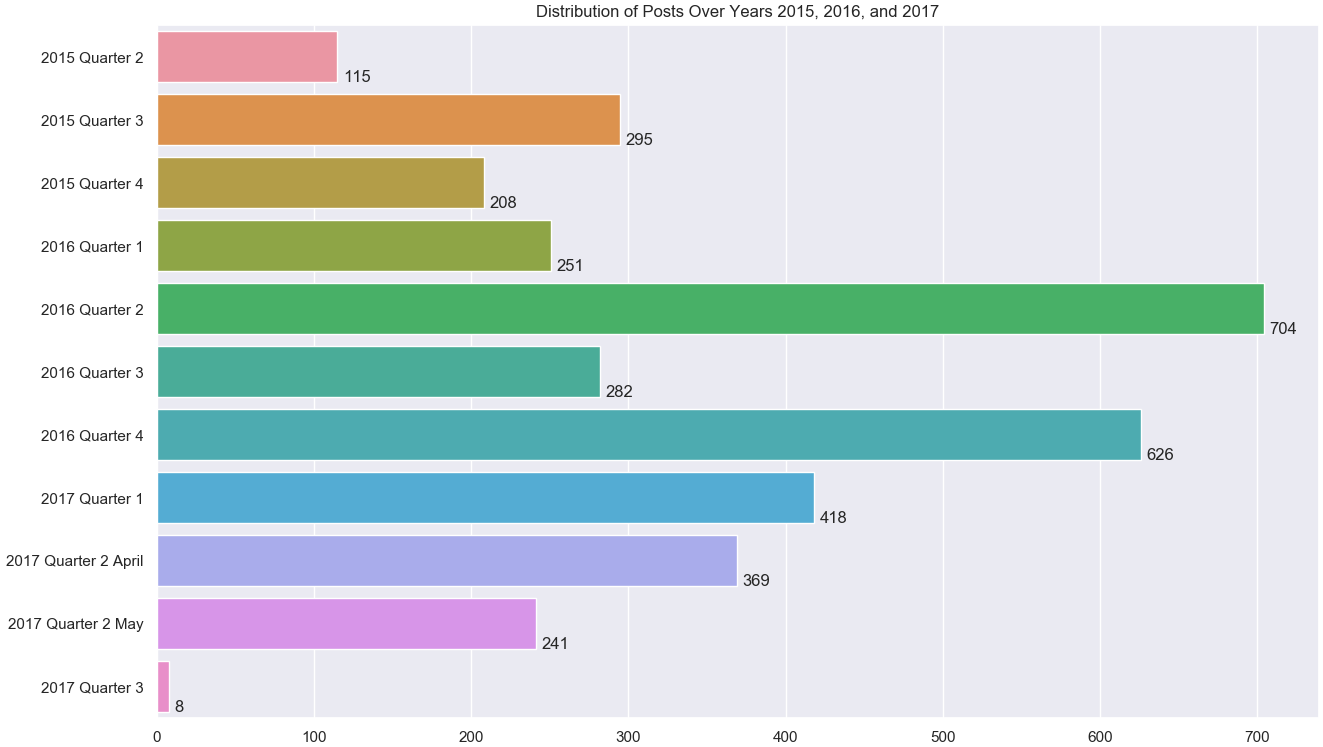
\includegraphics[width=0.75\columnwidth]{./image/barchart-plots/barchart_distribution_of_posts.png}
\caption*{Distribution of Posts Over Years 2015, 2016, and 2017.}
\end{figure}

As for ad spendings, the fourth quarter of 2016 exceeds that of any quarter,
with second quarter coming next. Interestingly, most of ads were paid in the
Russian currency (ruble) with two exceptions in 2016 quarter 3 and 2017 quarter
1 when IRA spent \$74.000 and \$35.330 respectively.

\begin{figure}[H]
\centering
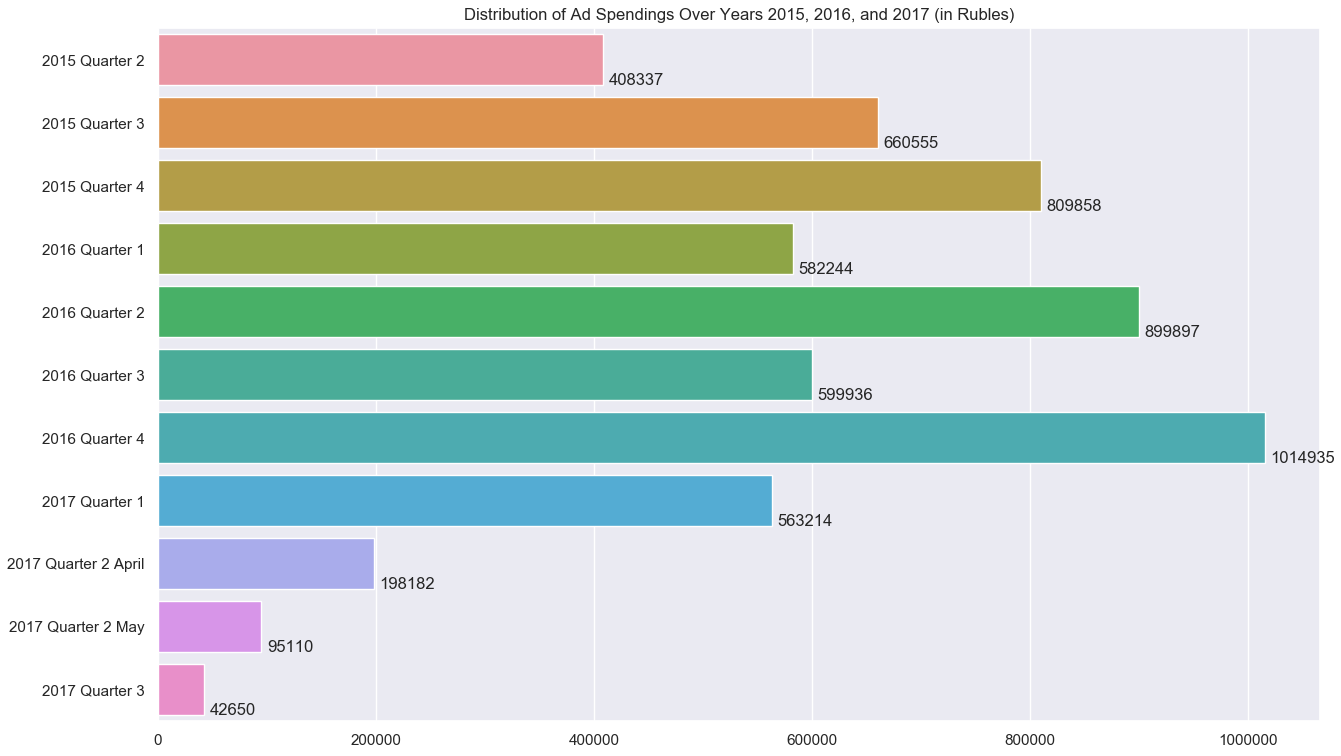
\includegraphics[width=0.75\columnwidth]{./image/barchart-plots/barchart_ad_spend_RU_distribution.png}
\caption*{Distribution of Ad Spendings Over Years 2015, 2016, and 2017 (in rubles).}
\end{figure}

Furthermore, 99.8\% of all paid ads across all years were paid in rubles.
Below is the chart showing the number of posts based on a currency.

\bigskip

\begin{center}
\begin{tabular}{|p{3cm}|p{3cm}|}
 \hline
 Currency & \text{Total (All Years)}\\
 \hline
 RUB  & 2549\\
 \hline
 USD  & 5\\
 \hline
 None & 787\\
 \hline
 0    & 176\\
 \hline
\end{tabular}
\end{center}

\bigskip

The Russian ruble is used in Russia, Belarus, and two regions of Georgia, which
are considered by Russia as partially recognised states of Abkhazia and South
Ossetia.

%%%%%%%%%%%%%%%%%%%%%%%%%%%%%%%%%%%%%%%%%%%%%%%%%%%%%%%%%%%%%%%%%%%%%%%%%%%%%%%
% Textual Analysis
%%%%%%%%%%%%%%%%%%%%%%%%%%%%%%%%%%%%%%%%%%%%%%%%%%%%%%%%%%%%%%%%%%%%%%%%%%%%%%%

\section*{\centering Textual Analysis}
\addcontentsline{toc}{section}{Textual Analysis}

\subsection*{\centering Common Words}
\addcontentsline{toc}{subsection}{Common Words}

Among the targeted approaches utilized by this campaign, one of the rather
noticeable ones was attacking the fissures of the United States by realizing
both social and political historical backgrounds.

\bigskip

Some of the most common words used in the campaign were black, police, and
people. Below is the barchart showing top 25 most commonly used words after
eliminating linking verbs, prepositions, pronouns, and some other
(non-relevant) words.

\begin{figure}[H]
\centering
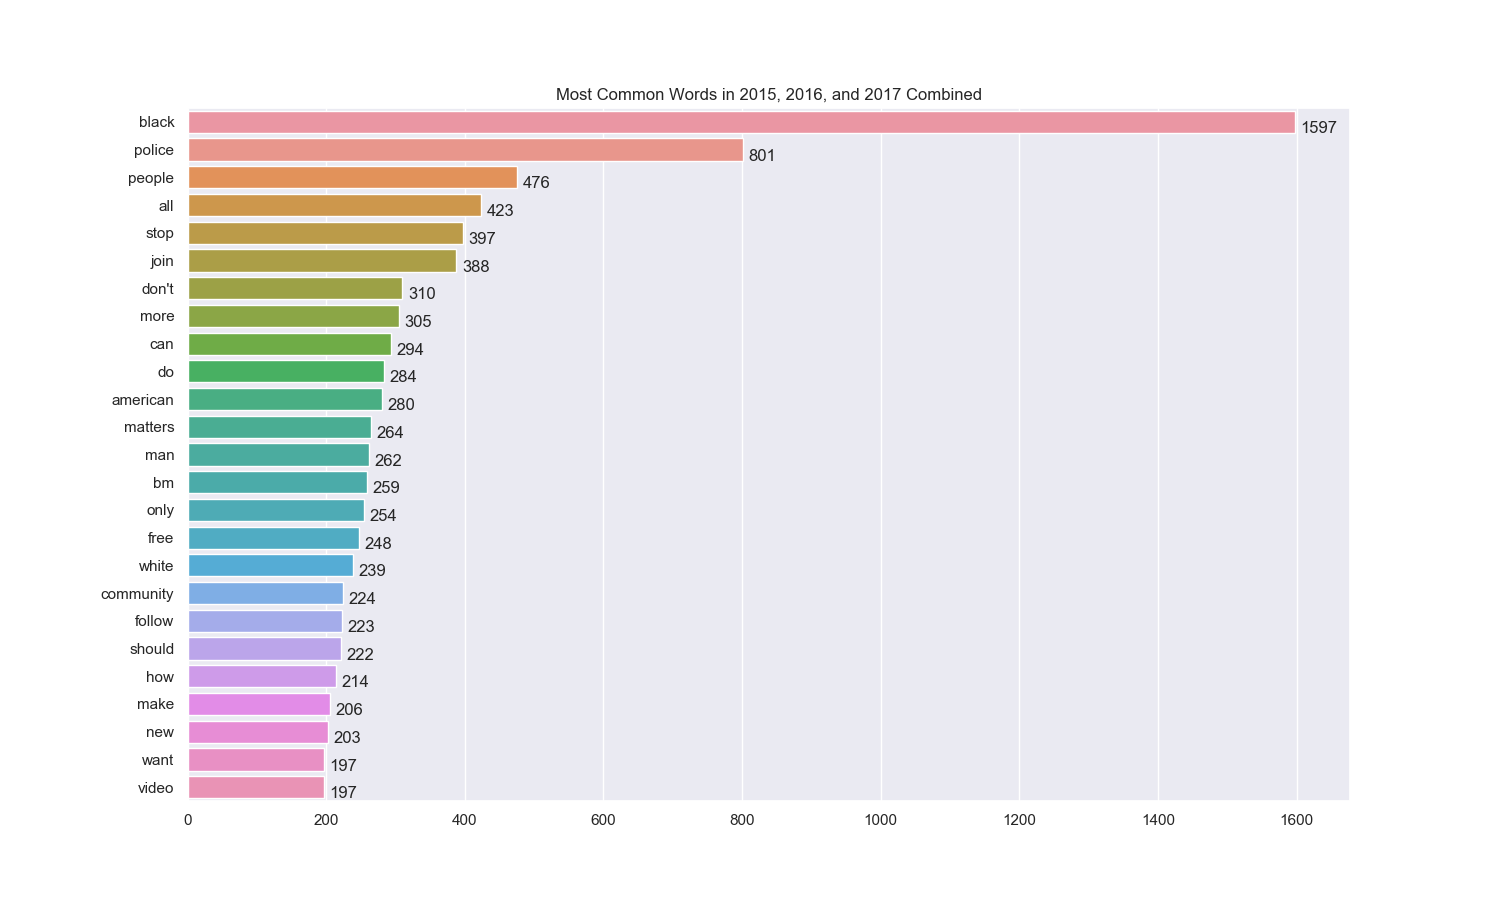
\includegraphics[width=\columnwidth]{./image/barchart-plots/barchart_word_counts.png}
\caption*{Figure.}
\end{figure}

%%%%%%%%%%%%%%%%%%%%%%%%%%%%%%%%%%%%%%%%%%%%%%%%%%%%%%%%%%%%%%%%%%%%%%%%%%%%%%%
% Sentiment Analysis
%%%%%%%%%%%%%%%%%%%%%%%%%%%%%%%%%%%%%%%%%%%%%%%%%%%%%%%%%%%%%%%%%%%%%%%%%%%%%%%

\subsubsection*{\centering Sentiment Analysis}
\addcontentsline{toc}{subsection}{Sentiment Analysis}
For the sentiment analysis purposes, we used \texttt{python}'s \texttt{TextBlob}
library. Suprisingly, out of all Facebook posts with \texttt{Ad Text}, 1643 were
positive, 900 negative, and 933 neutral leaving the overall tone of the posts
positive. Yet, the statistical significance of this claim is rather questionable
as the polarity levels were always near zero. Such low polarity level, however,
demonstrates a highly intelligent design of posts maximizing efficiency of
persuading targeted audience.

\bigskip

As the \texttt{Ad Text}s did not give us any strong proofs, we looked at the
negativity levels across all three years and found a consistent trend.

\bigskip

\begin{center}
\begin{tabular}{|p{3cm}|p{3cm}|p{3cm}|p{3cm}|p{3cm}|}
 \hline
 \multicolumn{5}{|c|}{Analyzing Negativity}\\
 \hline
 Subjectivity & Year 2015 & Year 2016 & Year 2017 & 2016 (\%)\\
 \hline
 1.0  & 154 & 562 & 176 & 63.004\\
 \hline
 0.75 & 150 & 547 & 169 & 63.164\\
 \hline
 0.5  & 123 & 405 & 120 & 62.500\\
 \hline
 0.25 & 15  & 81  & 22  & 68.644\\
 \hline
 0.15 & 5   & 33  & 10  & 68.750\\
 \hline
 0.1  & 2   & 11  & 6   & 57.895\\
 \hline
 0.05 & 1   & 5   & 2   & 62.500\\
 \hline
\end{tabular}
\end{center}

\bigskip

Notice that at any subjectivity level, year 2016 is consistently comprising
around 60\% of all posts. The year of the Presidentianl Election was rather
rather negative.

%%%%%%%%%%%%%%%%%%%%%%%%%%%%%%%%%%%%%%%%%%%%%%%%%%%%%%%%%%%%%%%%%%%%%%%%%%%%%%%
% Authorship Attribution
%%%%%%%%%%%%%%%%%%%%%%%%%%%%%%%%%%%%%%%%%%%%%%%%%%%%%%%%%%%%%%%%%%%%%%%%%%%%%%%

\subsubsection*{\centering Authorship Attribution}
\addcontentsline{toc}{subsection}{Authorship Attribution}

Since all of these posts were issued by the same political organization/entity,
it was interesting to see if there are some common patterns between the
Facebook ads of 2015, 2016, 2017. For this exact reason, we have performed
authorship attribution tests and have effectively implemented two
state-of-the art paper by Koppel et.~al.

%%%%%%%%%%%%%%%%%%%%%%%%%%%%%%%%%%%%%%%%%%%%%%%%%%%%%%%%%%%%%%%%%%%%%%%%%%%%%%%
% Bibliography and References
%%%%%%%%%%%%%%%%%%%%%%%%%%%%%%%%%%%%%%%%%%%%%%%%%%%%%%%%%%%%%%%%%%%%%%%%%%%%%%%

\newpage

\begin{center}
\printbibliography[heading=bibintoc]
\end{center}

%%%%%%%%%%%%%%%%%%%%%%%%%%%%%%%%%%%%%%%%%%%%%%%%%%%%%%%%%%%%%%%%%%%%%%%%%%%%%%%
% The end of the document
%%%%%%%%%%%%%%%%%%%%%%%%%%%%%%%%%%%%%%%%%%%%%%%%%%%%%%%%%%%%%%%%%%%%%%%%%%%%%%%

\end{document}
